\chapter{Overview and Descriptive Statistics}
\section{Populations, Samples, and Processes}
\begin{defn}
The \textbf{population} is the whole class of individuals which an investigator  is interested in.
\end{defn}

\begin{defn}
The \textbf{sample} is part of population which is examined or observed.
\end{defn}

From sample to population is what statistics do: chapter 6-16.

From population to sample is what probability do: chapter 2-5.
\begin{defn}
The \textbf{variable} is any characteristic whose value may change from one individual to another in population.
\end{defn}

\begin{exmp}
Household income; Examination score
\end{exmp}

In statistics, there are two important parts: Estimation and Influence.
\begin{itemize}
\item univariable one variable
\item bivariable two variables
\item multivariable more than two variables
\end{itemize}
\begin{exmp}
  77 100 52 78 95 55 86 43 86 73 89 68 57 85 58 79 90 45 95 46 85 77 98 86
  100 71 60 24 58 44 64 83 88 95 88 91 86 75 89 77 43 100 88 80 76 0 88 86
  69 44 40 84 68 87 86 83
\end{exmp}

\section{Pictorial and Tabular Methods in Descriptive Statistics}
\subsection{Stem-and-leaf plot}

\textbf{Procedure}

\begin{enumerate}
  \item select one or more leading digits as the \textbf{stems}. The tailing digits become the \textbf{leaves};
  \item List possible \textbf{stems} in a verticle column;
  \item List the \textbf{leaves} for every observation beside the corresponding \textbf{stem};
  \item Indicate the unit of \textbf{stems} and \textbf{leaves} in the plot.
\end{enumerate}

Therefore,
\begin{table}[H]
  \centering
  \caption{stem-and-leaf plot, Key: $1 | 1= 11$}
    \begin{tabular}{r|lllllllllllllllllll}
    0     & 0   \\
    1     \\
    2     & 4   \\
    3     \\
    4     & 0   & 3   & 3   & 4   & 4   & 5   & 6  \\
    5     & 2   & 5   & 7   & 8   & 8  \\
    6     & 0   & 4   & 8   & 8   & 9\\
    7     & 1   & 3   & 5   & 6   & 7   & 7   & 7   & 8   & 9   \\
    8     & 0   & 0   & 3   & 3   & 4   & 5   & 6   & 6   & 6   & 6   & 6   & 6   & 7   & 8   & 8   & 8   & 8   & 9   & 9  \\
    9     & 0   & 1   & 5   & 5   & 5   & 8   \\
    10    & 0   & 0   & 0 \\
    \end{tabular}
\end{table}


\subsection{Bar Plot}
Each observation is repeated as a dot above the corresponding location on a horizontal line with measurement scale.

\begin{figure}[htbp]
\centering
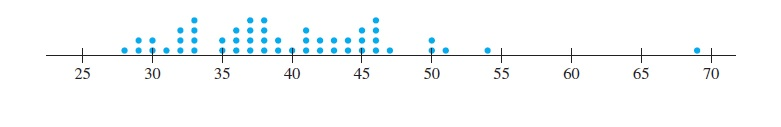
\includegraphics{figures/barplot.jpg}
\caption{A dotplot of the data from Example 1.8}
\label{fig:1}
\end{figure}


\subsection{Histogram}
\begin{defn}
A variable is \textbf{discrete} if its set of possible values either is finite or countable.
A variable is \textbf{continuous} if its set of possible values consists of an entire interval on the real line.
\end{defn}

\subsubsection{Discrete cases}

Frequency = number of times a value occur in the dataset.

Relative Frequency = $\frac{\text{\# of times the value occurs}}{\text{\# of observation in the dataset}}$
\vspace{4mm}

\textbf{Procedure}
\begin{enumerate}
  \item calculate the Frequency and Relative Frequency
  \item mark each value on a horizontal scale
  \item above each value, draw a rectangular whose height is the frequency or relative frequency of the value.
\end{enumerate}

\begin{figure}[H]
\centering
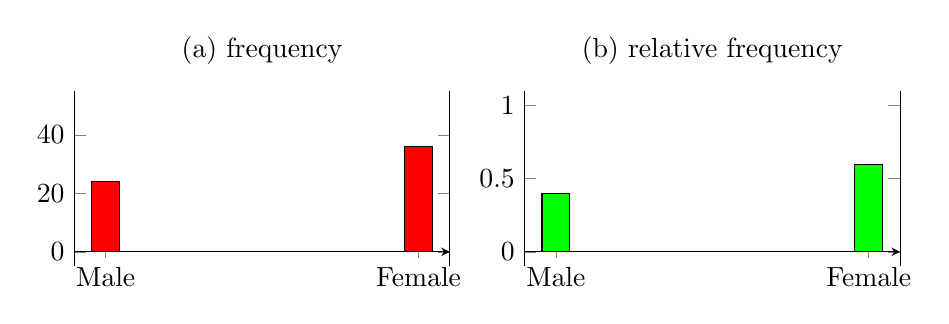
\begin{tikzpicture}
\begin{axis}[name =one,
width=2.5 in,
height=1.5in,
axis x line=center,
symbolic x coords={Male,Female},
xtick=data,
title= (a) frequency,
enlargelimits=true,
ymin=0, ymax=50,
]
\addplot[ybar,fill=red] coordinates {
	(Male,   24)
	(Female, 36)
	};
%amd
\end{axis}

\begin{axis}[name=two,at=(one.right of south east), anchor=left of south west,
width=2.5in,
height=1.5in,
axis x line=center,
symbolic x coords={Male,Female},
xtick=data,
title= (b) relative frequency,
enlargelimits=true,
ymin=0, ymax=1,
]
\addplot[ybar,fill=green] coordinates {
	(Male,   0.4)
	(Female, 0.6)
	};
%nvidia
\end{axis}
\end{tikzpicture}

\end{figure}

\subsubsection{Continuous cases}
Need to determine the size of each class.

\textbf{(a) Equal class}: similar to discrete case.

\begin{figure}[H]
\centering
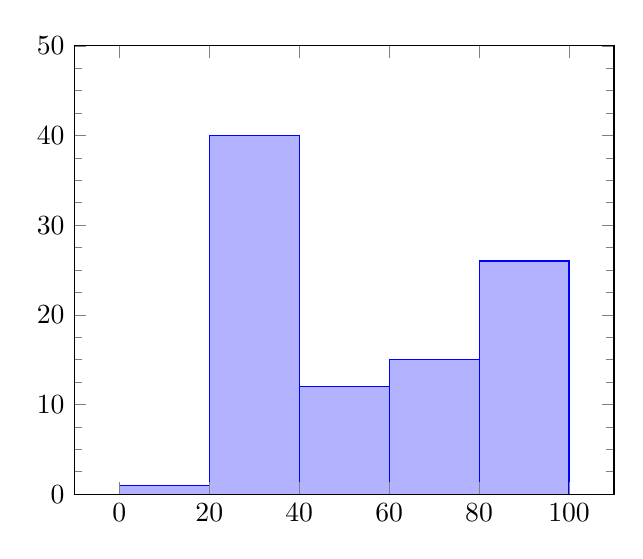
\begin{tikzpicture}
\begin{axis}[
    ymin=0, ymax=50,
    minor y tick num = 3,
    area style,
    ]
\addplot+[ybar interval,mark=no] plot coordinates { (0,1 ) (20, 40) (40, 12) (60,15) (80, 26) (100, 0) };
\end{axis}
\end{tikzpicture}
\end{figure}


You can also use the relative frequency.


\textbf{(b) The unequal class}:
\begin{exmp}
  0-10K, 10K-20K, 20-30K, \dots, 500K-510K, 510K-520K, \dots 
  (a waste of space!) 
  
  $\Rightarrow $  0-10K, 10K-20K, 20K-30K, 30K-40K, 40K-50K,  50K-100K, 100K-200K
\end{exmp}
For the unequal class, frequency or relative frequency may mislead some people because of a wide range. Therefore, we use density.
\[ \text{Density} = \frac{\text{relative frequency of the class}}{\text{class width}}
\]
Use density as height to draw histogram within unequal class.
\subsubsection{Shape of histogram}
\begin{itemize}
  \item Mode: unimodal, bimodal, multimodal
  \item Symmetry: symmetric, positive skewed, negative skewed
\end{itemize}

\begin{figure}[H]
\centering
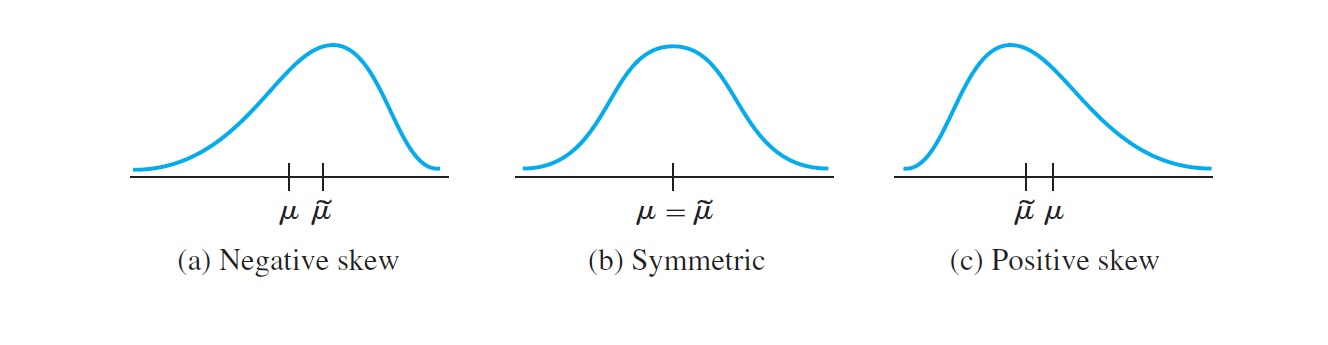
\includegraphics{figures/shape_histogram.jpg}
\caption{Three different shapes for a population distribution}
\label{fig:2}
\end{figure}

\section{Measures of Location and Variability}
\subsection{Location}

Observations: \[x_1,x_2 \dots x_n\]

Sample mean:
\[\bar{x}=\frac{\sum_{i=1}^{n} x_i}{n}\]

Sample median:
\[
\tilde{x}=\begin{cases}
\frac{n+1}{2}\text{th ordered value}, &\text{if n is odd}\\
\frac{n}{2}\text{ or }\frac{n+2}{2}\text{th ordered value}. &\text{if n is even}
\end{cases}\]


\begin{itemize}
  \item symmetric: $x\approx \tilde{x}$
  \item positive skewed: $x>\tilde{x}$
  \item negative skewed: $x<\tilde{x}$
\end{itemize}

If you want your mean closer to your sample median. You can use \textbf{truncated mean}.


\subsection{Variability}
\begin{exmp}
Two dataset
  \begin{itemize}
    \item Dataset 1 \qquad 1,100 \qquad  $\bar{x}=50.5$ \qquad $\tilde{x}=50.5$
    \item Dataset 2 \qquad 50,51 \qquad  $\bar{x}=50.5$ \qquad $\tilde{x}=50.5$
  \end{itemize}
\end{exmp}


\vspace{4mm}
Sample Variance: \[S^2=\frac{\sum_{i=1}^{n} (x_i-\bar{x})^2}{n-1}\]

Sample Standard deviation (s.d): $S=\sqrt{S^2}$

\vspace{4mm}

Short-cut formula:
\[S^2=\frac{{\sum_{i=1}^{n} x_i^2} - n{\bar{x}}^2}{n-1}
\]
\begin{proof}
\[\sum_{i=1}^{n}(x_i-\bar{x})^2=
\sum_{i=i}^{n}(x_i^2+2x_i\bar{x}+{\bar{x}}^2)=
\sum_{i=i}^{n}x_i^2-2\bar{x}\sum_{i=1}^{n}x_i+
\sum_{i=i}^{n}\bar{x}^2 \]
Since \[\bar{x}=\frac{\sum_{i=1}^{n} x_i}{n}, \qquad n\bar{x}=\sum_{i=1}^{n} x_i \]
Substitute this, and the proof is done. 
\end{proof}

\begin{prop}
  Let $x_1 \dots x_n$ be a sample, and $c$ be any nonzero constant.
  \begin{enumerate}
    \item Let $y_1=x_1+c,y_2=x_2+c,\dots,y_n=x_n+c$, then
    \[\bar{y}=\bar{x}+c, S_y^2=S_x^2\]
    \item Let $z_1=cx_1,z_2=cx_2,\dots,z_n=cx_n$, then
    \[\bar{z}=c \bar{x}, S_z^2=c^2S_z^2\]
    \end{enumerate}
\end{prop}

\subsection{Boxplot}
The simplest boxplot is based on the following five-number summary:

smallest $x_i$, \quad lower fourth,\quad median, \quad upper fourth, \quad largest $x_i$
\begin{defn}
  Any observation farther than 1.5$f_s$ from the closest fourth is an \textbf{outlier}. An outlier is \textbf{extreme} if it is more than 3$f_s$ from the nearest fourth, and it is \textbf{mild} otherwise.
\end{defn}

Each mild outlier is represented by a closed circle and each extreme outlier by an open circle.

\begin{figure}[H]
\centering
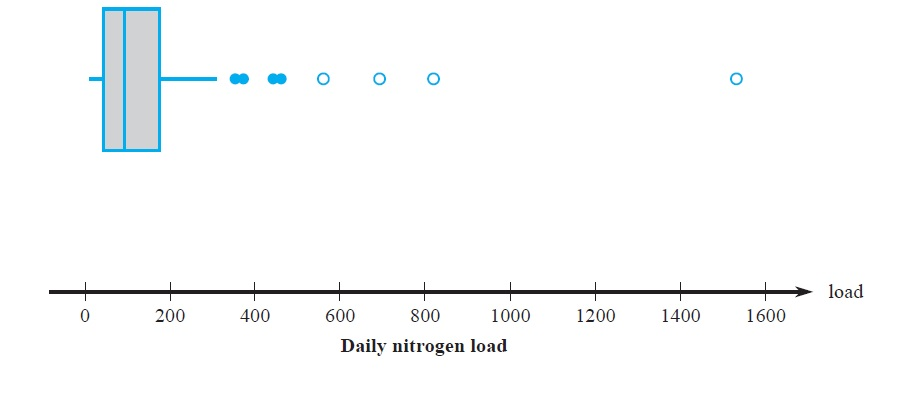
\includegraphics{figures/boxplot.jpg}
\caption{Boxplots That Show Outliers}
\label{fig:3}
\end{figure}